\documentclass[../notes.tex]{subfiles}

\pagestyle{main}
\renewcommand{\chaptermark}[1]{\markboth{\chaptername\ \thechapter\ (#1)}{}}
\setcounter{chapter}{14}

\begin{document}




\chapter{Light-Matter Interactions}
\section{Photochemistry}
\begin{itemize}
    \item \marginnote{12/10:}Announcements.
    \begin{itemize}
        \item Alex plugs the course evaluations again.
        \item No class Thursday.
        \item On the exam.
        \begin{itemize}
            \item They wrote the exam, intending for it to be difficult. Alex and Masha respect us as chemists, and wanted to challenge us to explore our full potentials.
            \item Regardless of how you did on the exam, if you engaged it seriously, you succeeded per Alex.
            \item No single exam is a referendum on our value as a chemist or worth as a human.
            \item If it didn't go as planned, feel free to reach out to Alex, Masha, or anybody else in the chemical faculty if you feel that they can help you learn something. We are all in a place of mutual learning, and you should take advantage of that opportunity.
        \end{itemize}
        \item On the mechanistic proposal.
        \begin{itemize}
            \item Jonathan grades Exam 2; Alex grades the mechanistic proposal.
            \item They will get our grades back to us before the deadline to submit/lock in grades.
        \end{itemize}
    \end{itemize}
    \item Today: Light-matter interactions (the photophysics and photochemistry of organic molecules).
    \begin{itemize}
        \item This is an addendum to electron transfer.
        \item In an ideal world, organic photochemistry would not be a final lecture in 5.53; it would be a half- or full-semester course. But alas, they don't have that in the syllabus.
        \item Hopefully this gives us some useful context to approach the literature with greater insight, though.
    \end{itemize}
    \item Consider an atom with a spherically symmetric electron distribution.
    \begin{figure}[H]
        \centering
        \begin{subfigure}[b]{0.42\linewidth}
            \centering
            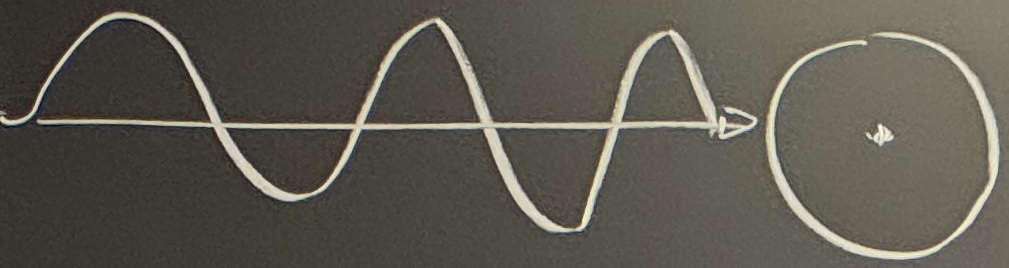
\includegraphics[width=0.43\linewidth]{lightAtoma.JPG}
            \caption{Impinging photon.}
            \label{fig:lightAtoma}
        \end{subfigure}
        \begin{subfigure}[b]{0.42\linewidth}
            \centering
            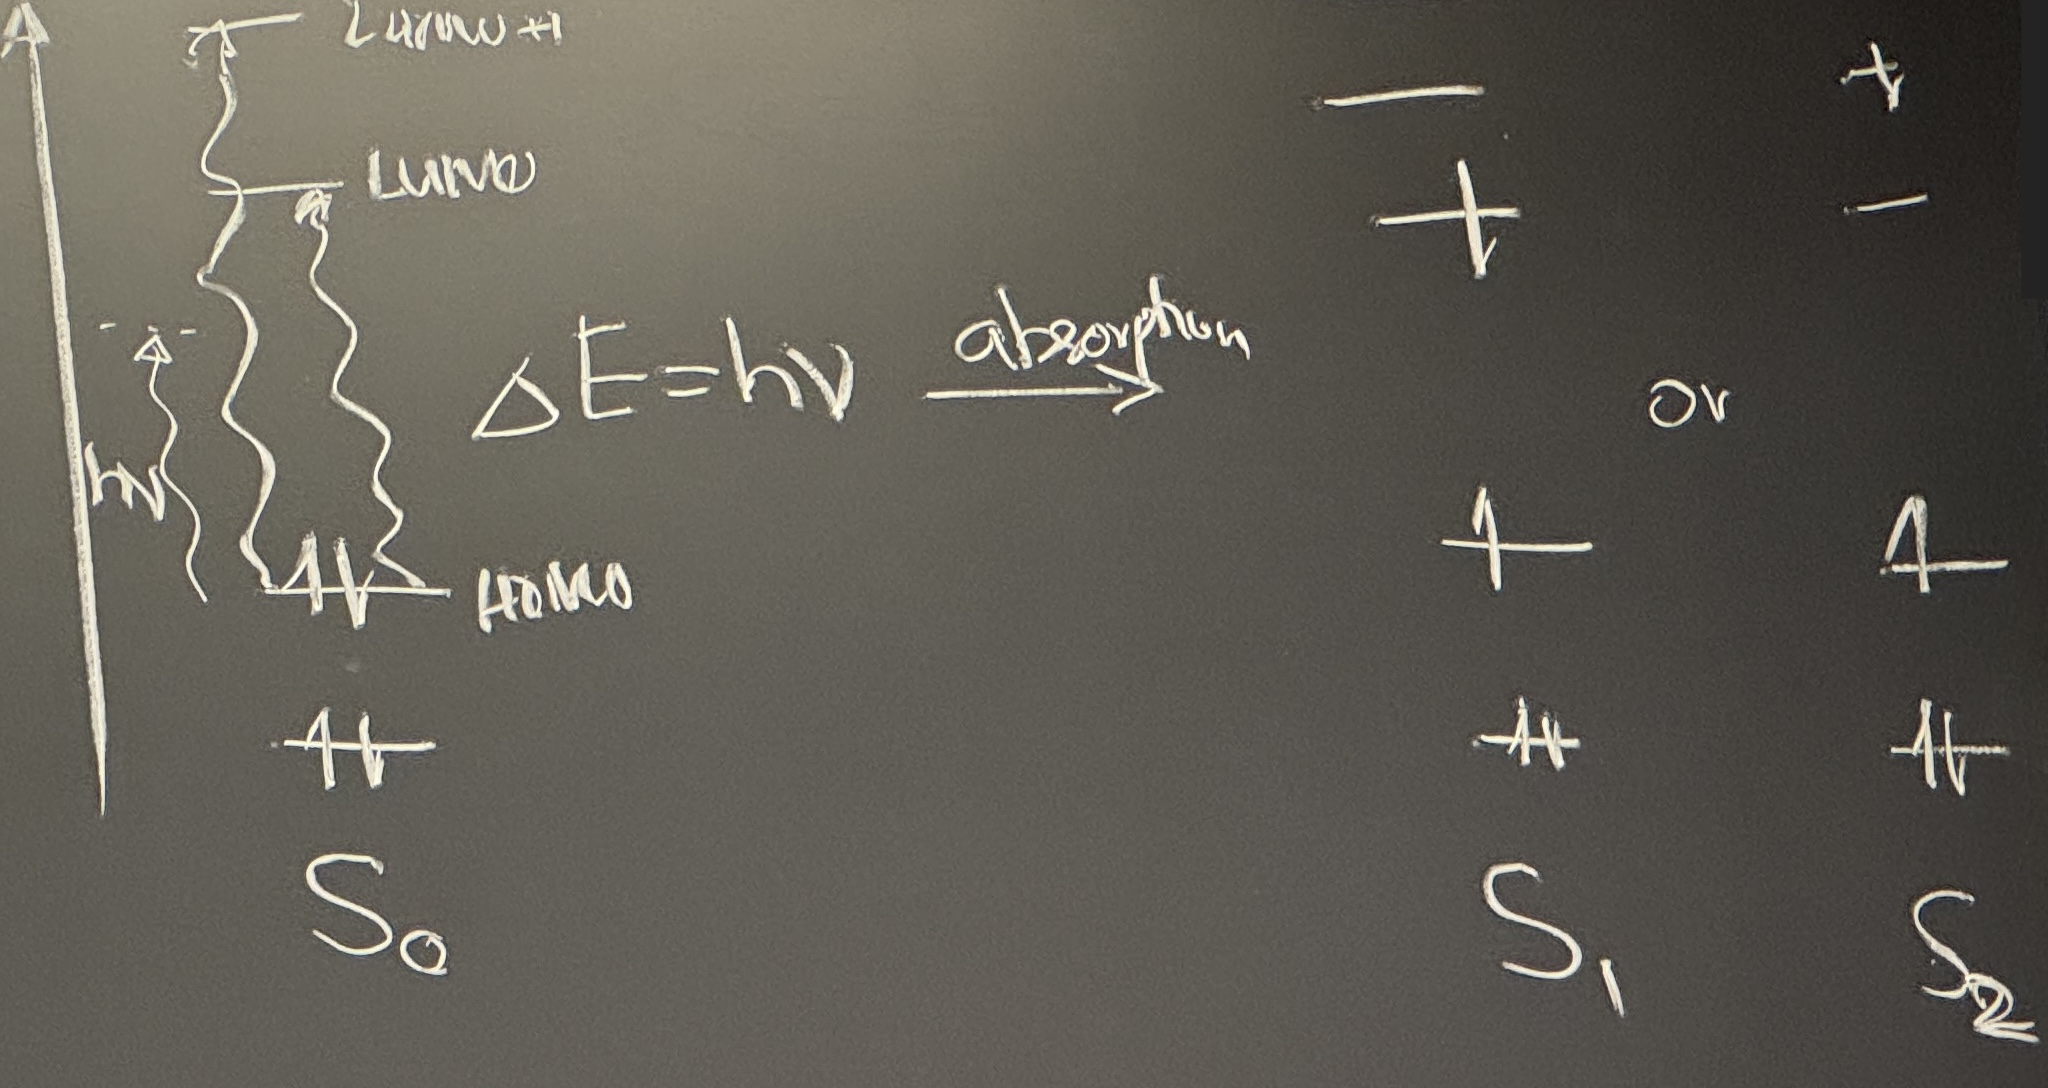
\includegraphics[width=0.95\linewidth]{lightAtomb.JPG}
            \caption{Orbital effects.}
            \label{fig:lightAtomb}
        \end{subfigure}
        \caption{Irradiation of an atom with light.}
        \label{fig:lightAtom}
    \end{figure}
    \begin{itemize}
        \item Suppose we impinge upon the atom with \textbf{light}.
        \item Electrons are charged particles, and thus will interact with the light.
        \item A bunch of stuff can happen, depending on the energy/wavelength/frequency of the light.
        \begin{equation*}
            E = h\nu
            = \frac{hc}{\lambda}
        \end{equation*}
        \item Suppose that this atom has some electrons in filled orbitals, and some possible stable electronic states/wavefunctions defined by the nuclear potential.
        \item If you have a photon of random energy (not corresponding to any orbital gab), it will create a nearly instantaneous virtual state.
        \begin{itemize}
            \item The atom can elastically or inelastically scatter the photon.
            \item Inelastic scattering is the basis for Raman spectroscopy!
        \end{itemize}
        \item The transit of the photon through the electron cloud can also meet a resonance condition between the energies of the wave functions.
        \begin{itemize}
            \item This does not lead to scattering of the photon, but to to \emph{absorption} of the photon.
        \end{itemize}
        \item Because reasons, the spin angular momentum of the electron will not be affected by this absorption.
        \item The ground state is $S_0$ (a singlet, ground state).
        \begin{itemize}
            \item The excited state is $S_1$ (still a singlet, but no longer a ground state).
            \item A doubly excited singlet state is $S_2$.
        \end{itemize}
    \end{itemize}
    \item \textbf{Light}: An oscillating electromagnetic field traversing the universe.
    \item Let's now look at the effect of this excitation on a molecule.
    \begin{figure}[h!]
        \centering
        \begin{subfigure}[b]{0.49\linewidth}
            \centering
            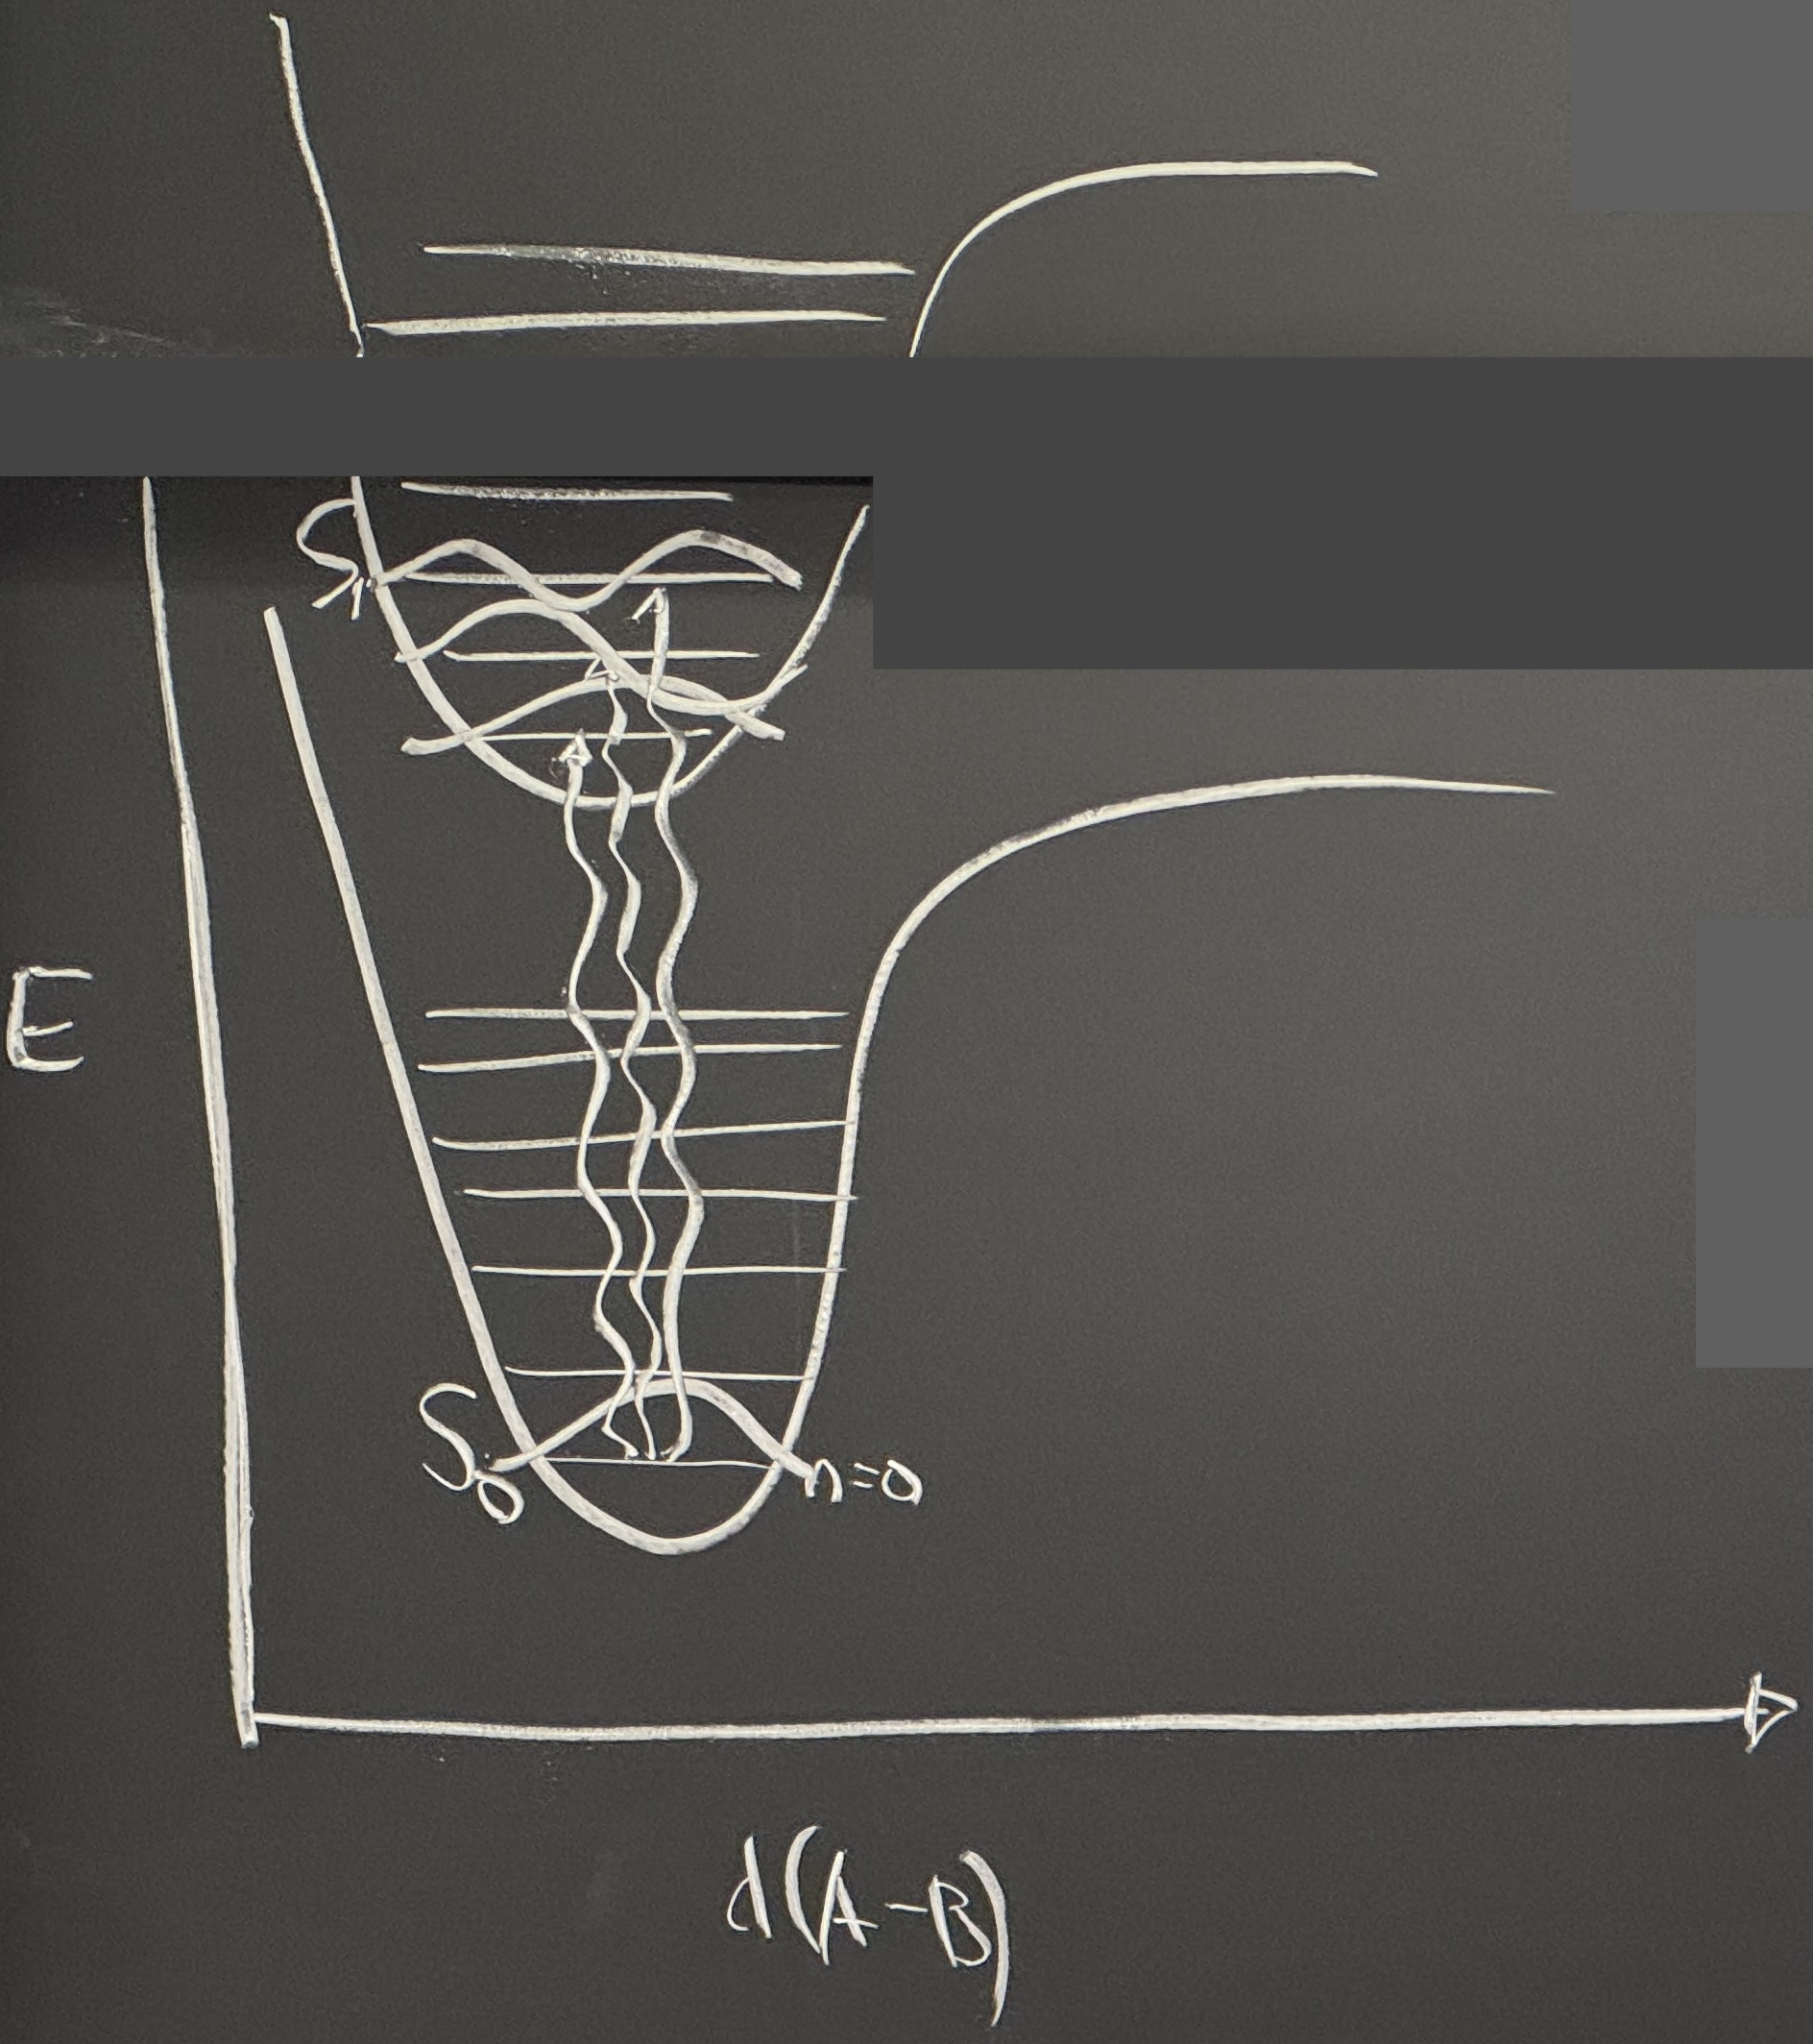
\includegraphics[width=0.8\linewidth]{lightMolSimplea.JPG}
            \caption{Electronic promotion potential energy surfaces.}
            \label{fig:lightMolSimplea}
        \end{subfigure}
        \begin{subfigure}[b]{0.35\linewidth}
            \centering
            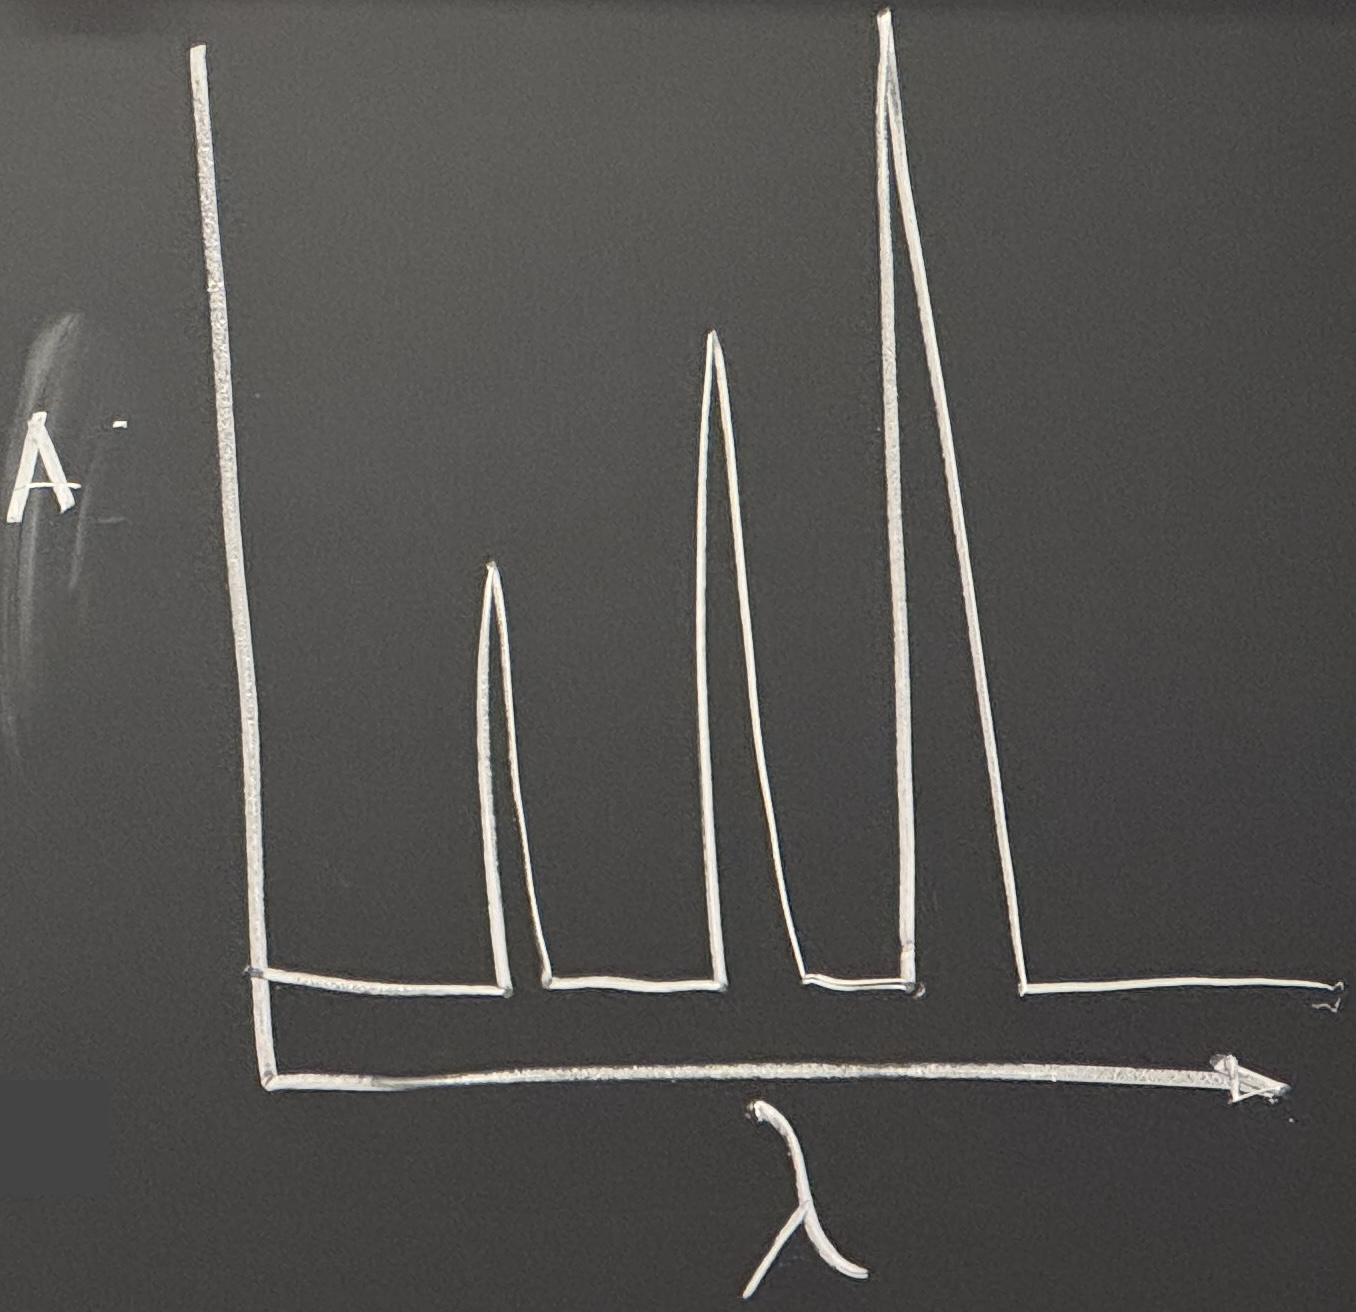
\includegraphics[width=0.8\linewidth]{lightMolSimpleb.JPG}
            \caption{Vibrational spectrum.}
            \label{fig:lightMolSimpleb}
        \end{subfigure}
        \caption{Irradiation of a molecule with light (simplistic).}
        \label{fig:lightMolSimple}
    \end{figure}
    \begin{itemize}
        \item The higher-lying vibrational states (in $S_0$) will be populated via a Boltzmann distribution.
        \item When we excite into $S_1$, we jump to a different potential energy surface (Figure \ref{fig:lightMolSimplea})!
        \item We can also array absorption vs. wavelength (Figure \ref{fig:lightMolSimpleb}).
        \begin{itemize}
            \item Slightly different photons can excite into higher vibrational states.
            \item We expect more absorption of lower energy photons because there is greater orbital overlap of the $S_0$ ($n=0$) state with the $S_1$ ($n=0$) state than with any of the $S_1$ ($n>0$) states.
        \end{itemize}
    \end{itemize}
    \pagebreak
    \item The energy range for these excitations is usually in the UV-Vis range.
    \begin{itemize}
        \item Visible irradiation: \SIrange{400}{700}{\nano\meter} is equivalent to \kcalr{75}{45} of energy.
        \item UV irradiation: \SIrange{200}{400}{\nano\meter} is equivalent to \kcalr{150}{75} of energy.
    \end{itemize}
    \item Modifying this picture.
    \begin{figure}[h!]
        \centering
        \begin{subfigure}[b]{0.49\linewidth}
            \centering
            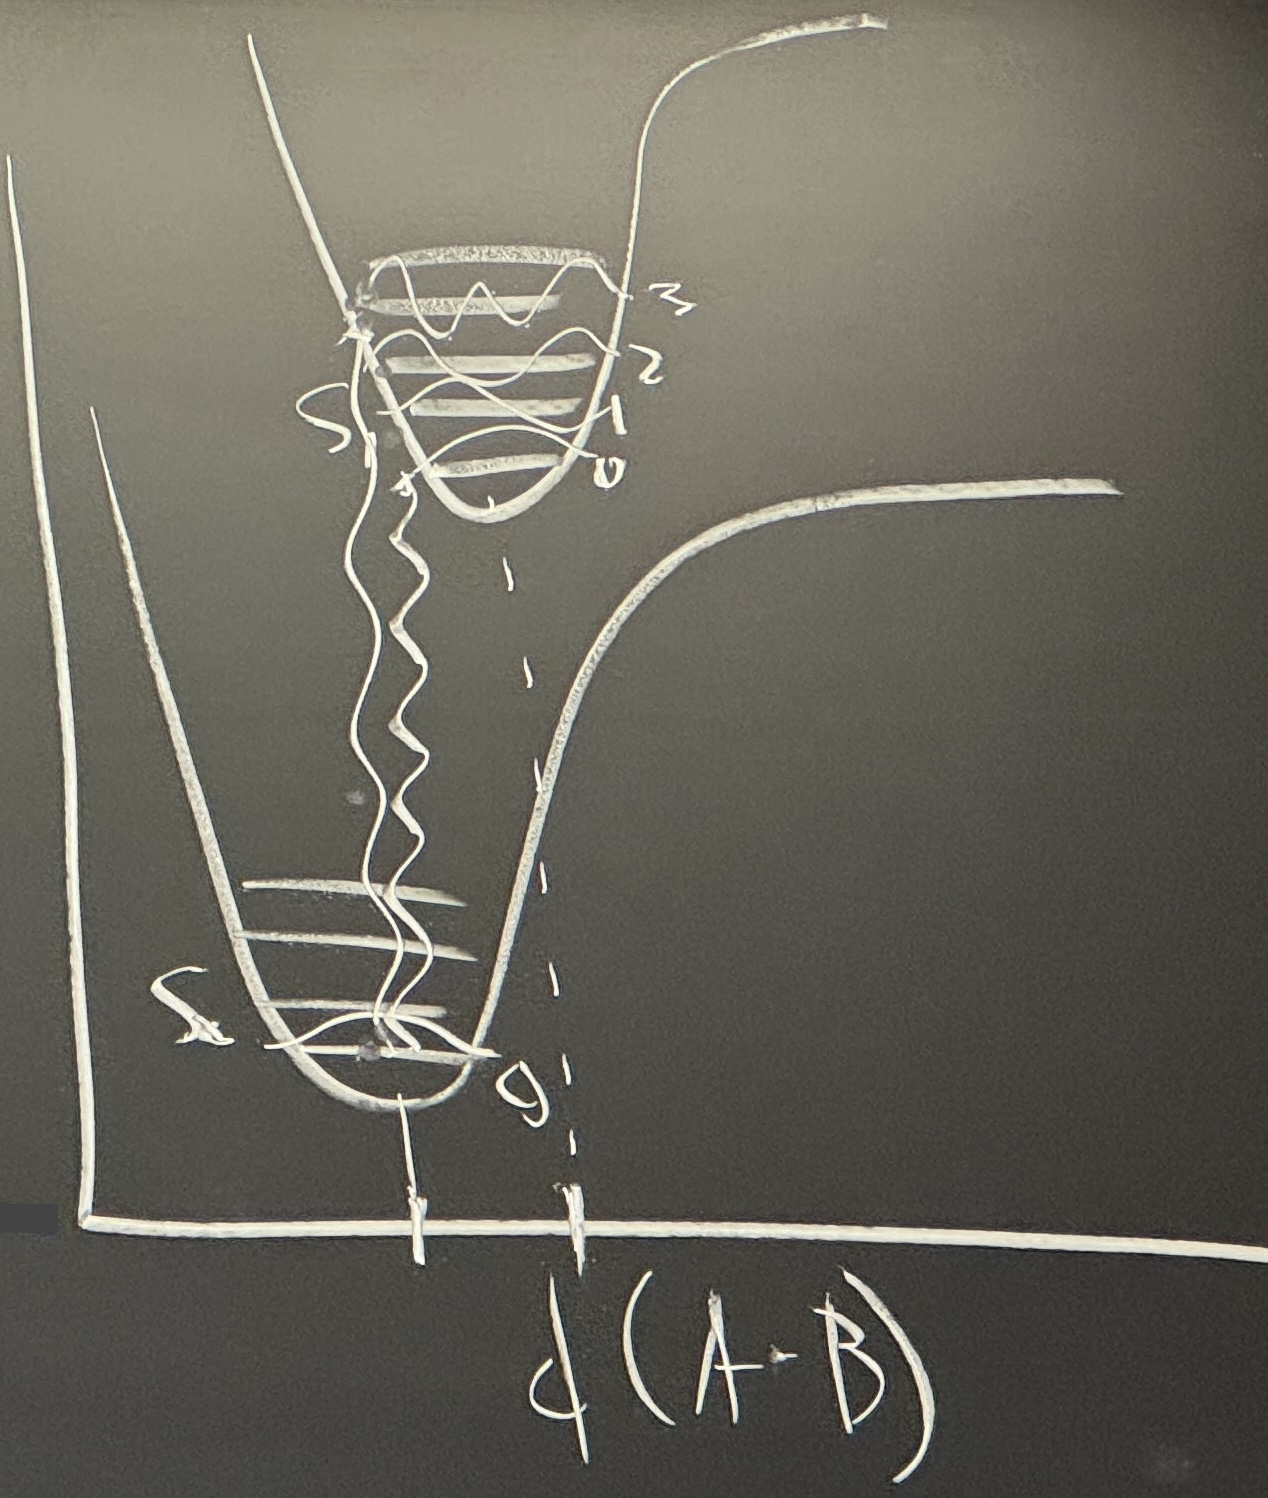
\includegraphics[width=0.65\linewidth]{lightMola.JPG}
            \caption{Electronic promotion potential energy surfaces.}
            \label{fig:lightMola}
        \end{subfigure}
        \begin{subfigure}[b]{0.35\linewidth}
            \centering
            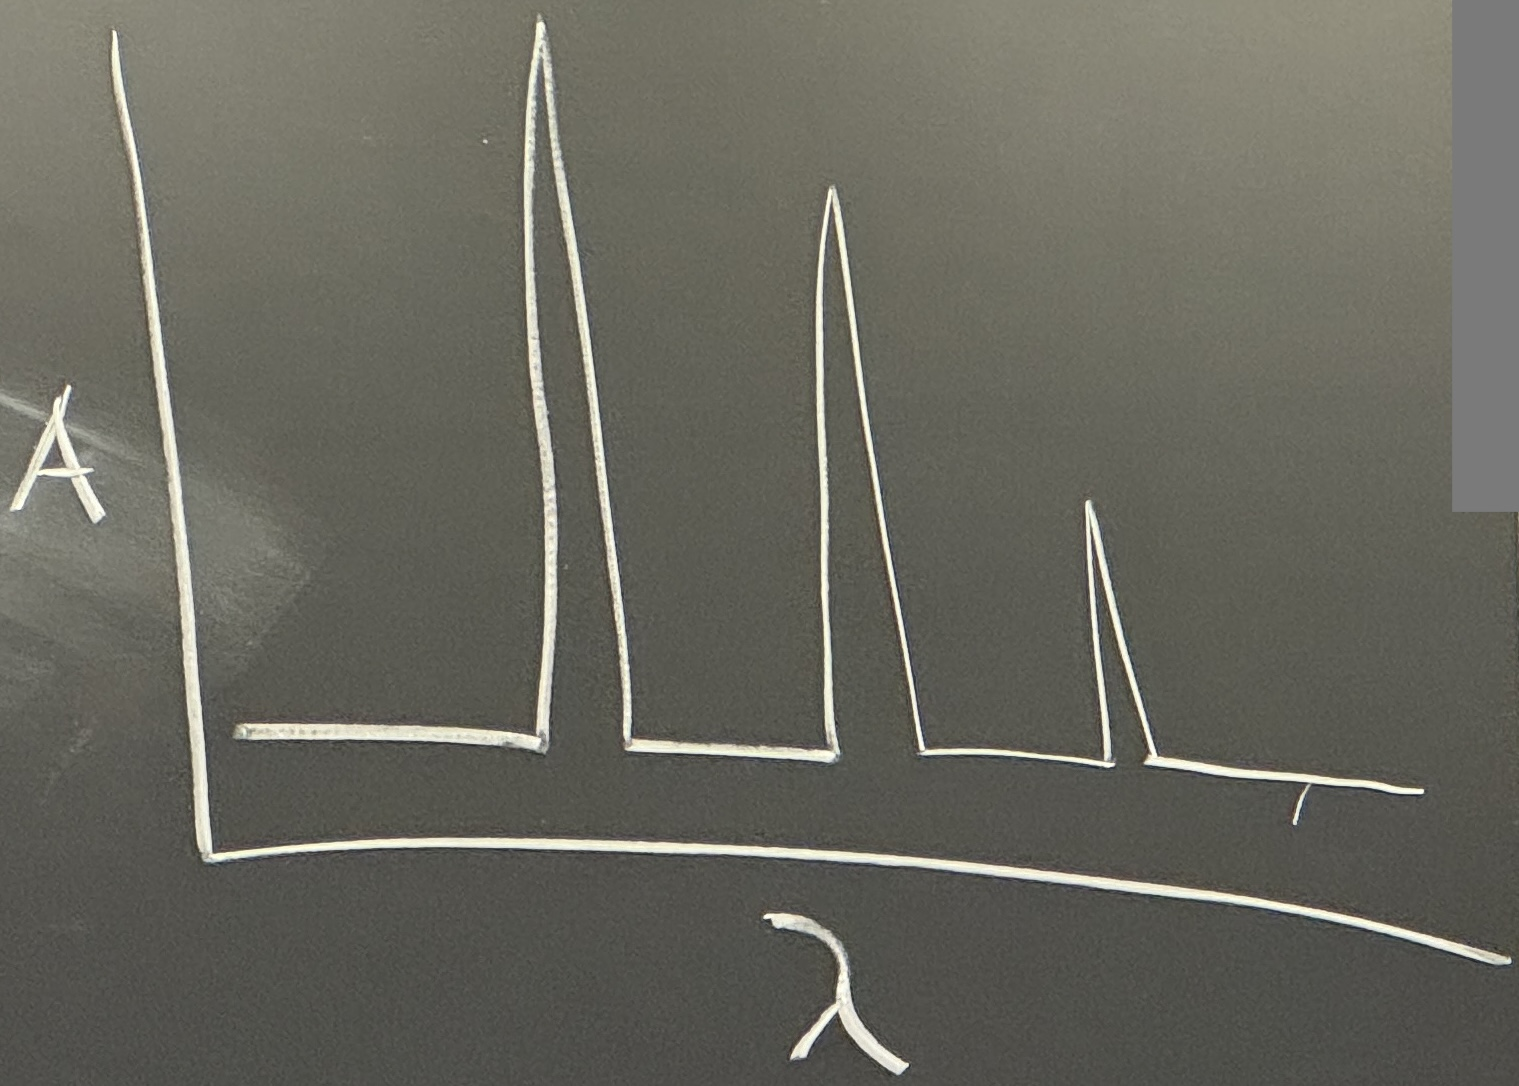
\includegraphics[width=0.8\linewidth]{lightMolb.JPG}
            \caption{Vibrational spectrum.}
            \label{fig:lightMolb}
        \end{subfigure}
        \caption{Irradiation of a molecule with light (real).}
        \label{fig:lightMol}
    \end{figure}
    \begin{itemize}
        \item It's not that the excited electron spends less time between the nuclei; that's too classical.
        \begin{itemize}
            \item Rather, population of higher-energy, antibonding orbitals leads to decreased bond order in the excited state that shifts the $S_1$ potential energy surface over to the right.
        \end{itemize}
        \item This leads to the \textbf{Franck-Condon principle}, which implies that peak distribution flips.
    \end{itemize}
    \item \textbf{Franck-Condon principle}: Electronic transitions proceed vertically, irrespective of nuclear motion.
    \begin{itemize}
        \item Like Born-Oppenheimer, electrons are assumed to move on a timescale where nuclei stand still.
        \item Also reflects that we like exciting into wave functions having more overlap with the ground state.
    \end{itemize}
    \item Once a molecule is excited, what happens? There are several mechanisms of relaxation.
    \begin{figure}[H]
        \centering
        \begin{subfigure}[b]{0.33\linewidth}
            \centering
            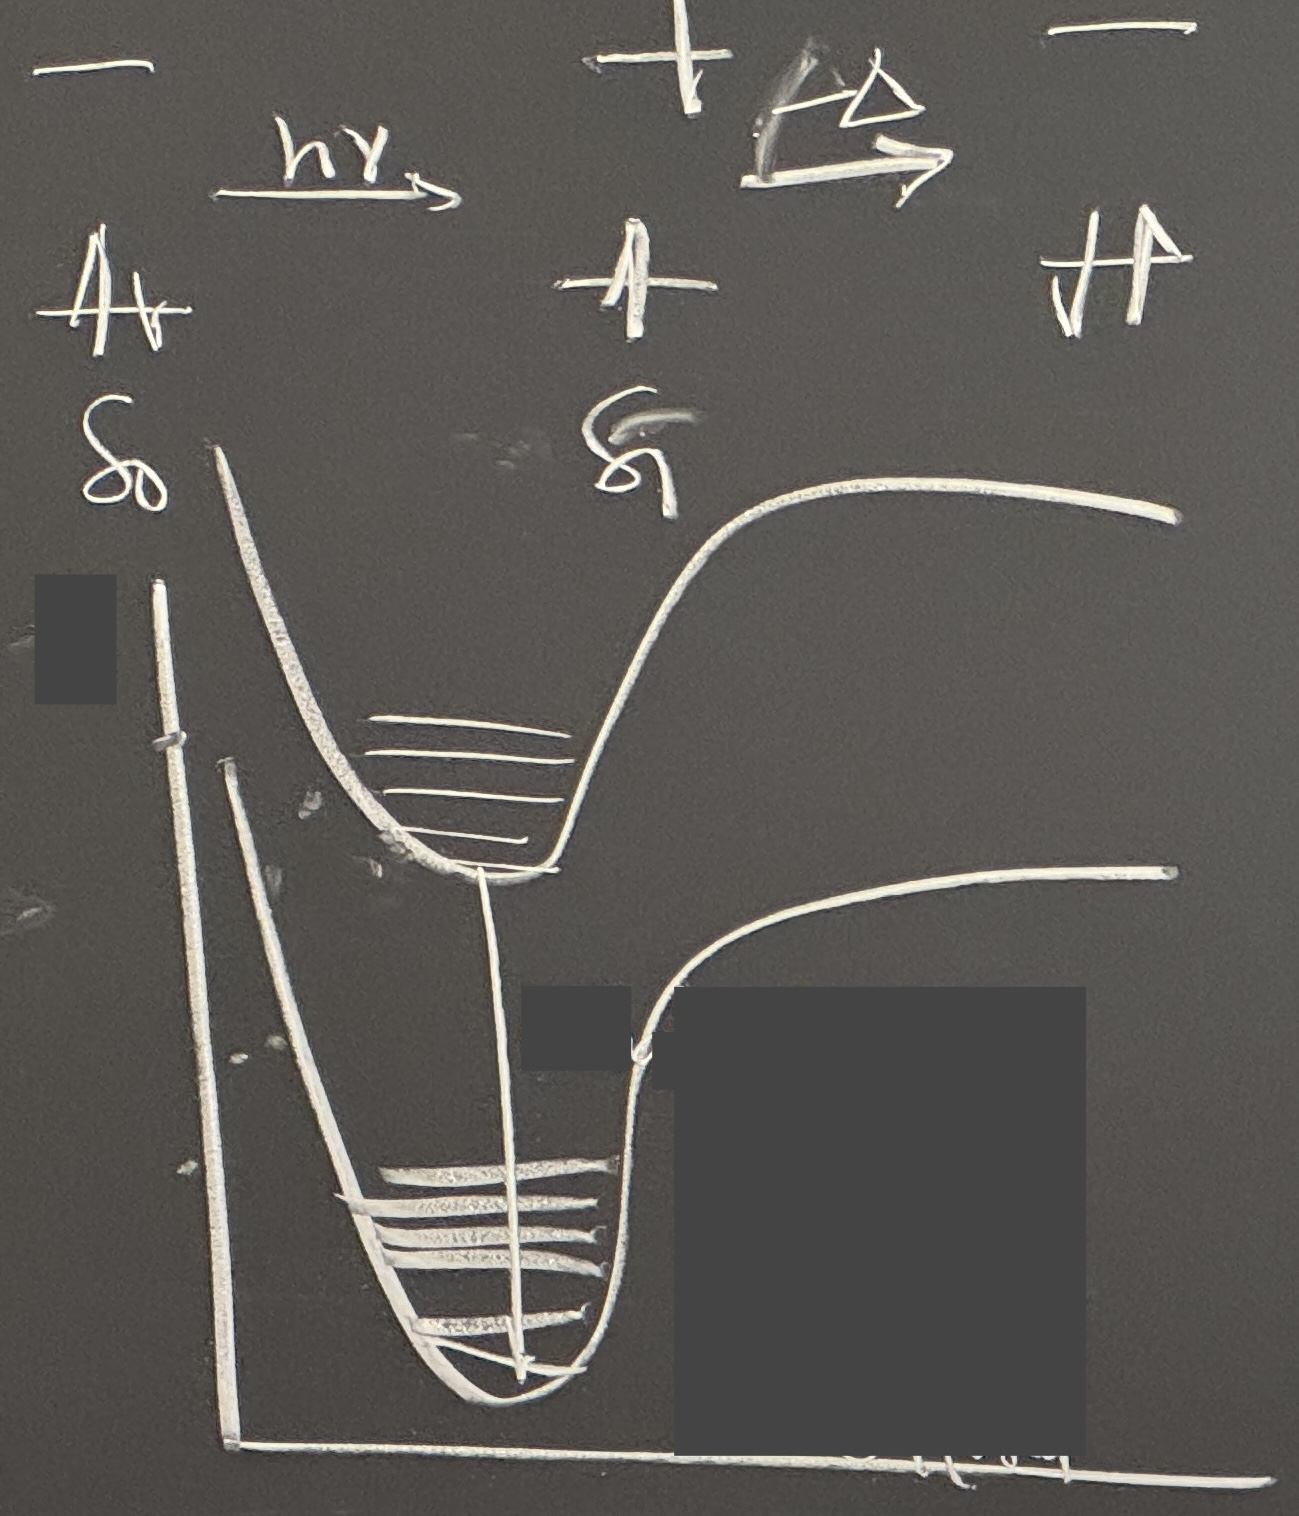
\includegraphics[width=0.85\linewidth]{relaxationMecha.JPG}
            \caption{Internal conversion.}
            \label{fig:relaxationMecha}
        \end{subfigure}
        \begin{subfigure}[b]{0.32\linewidth}
            \centering
            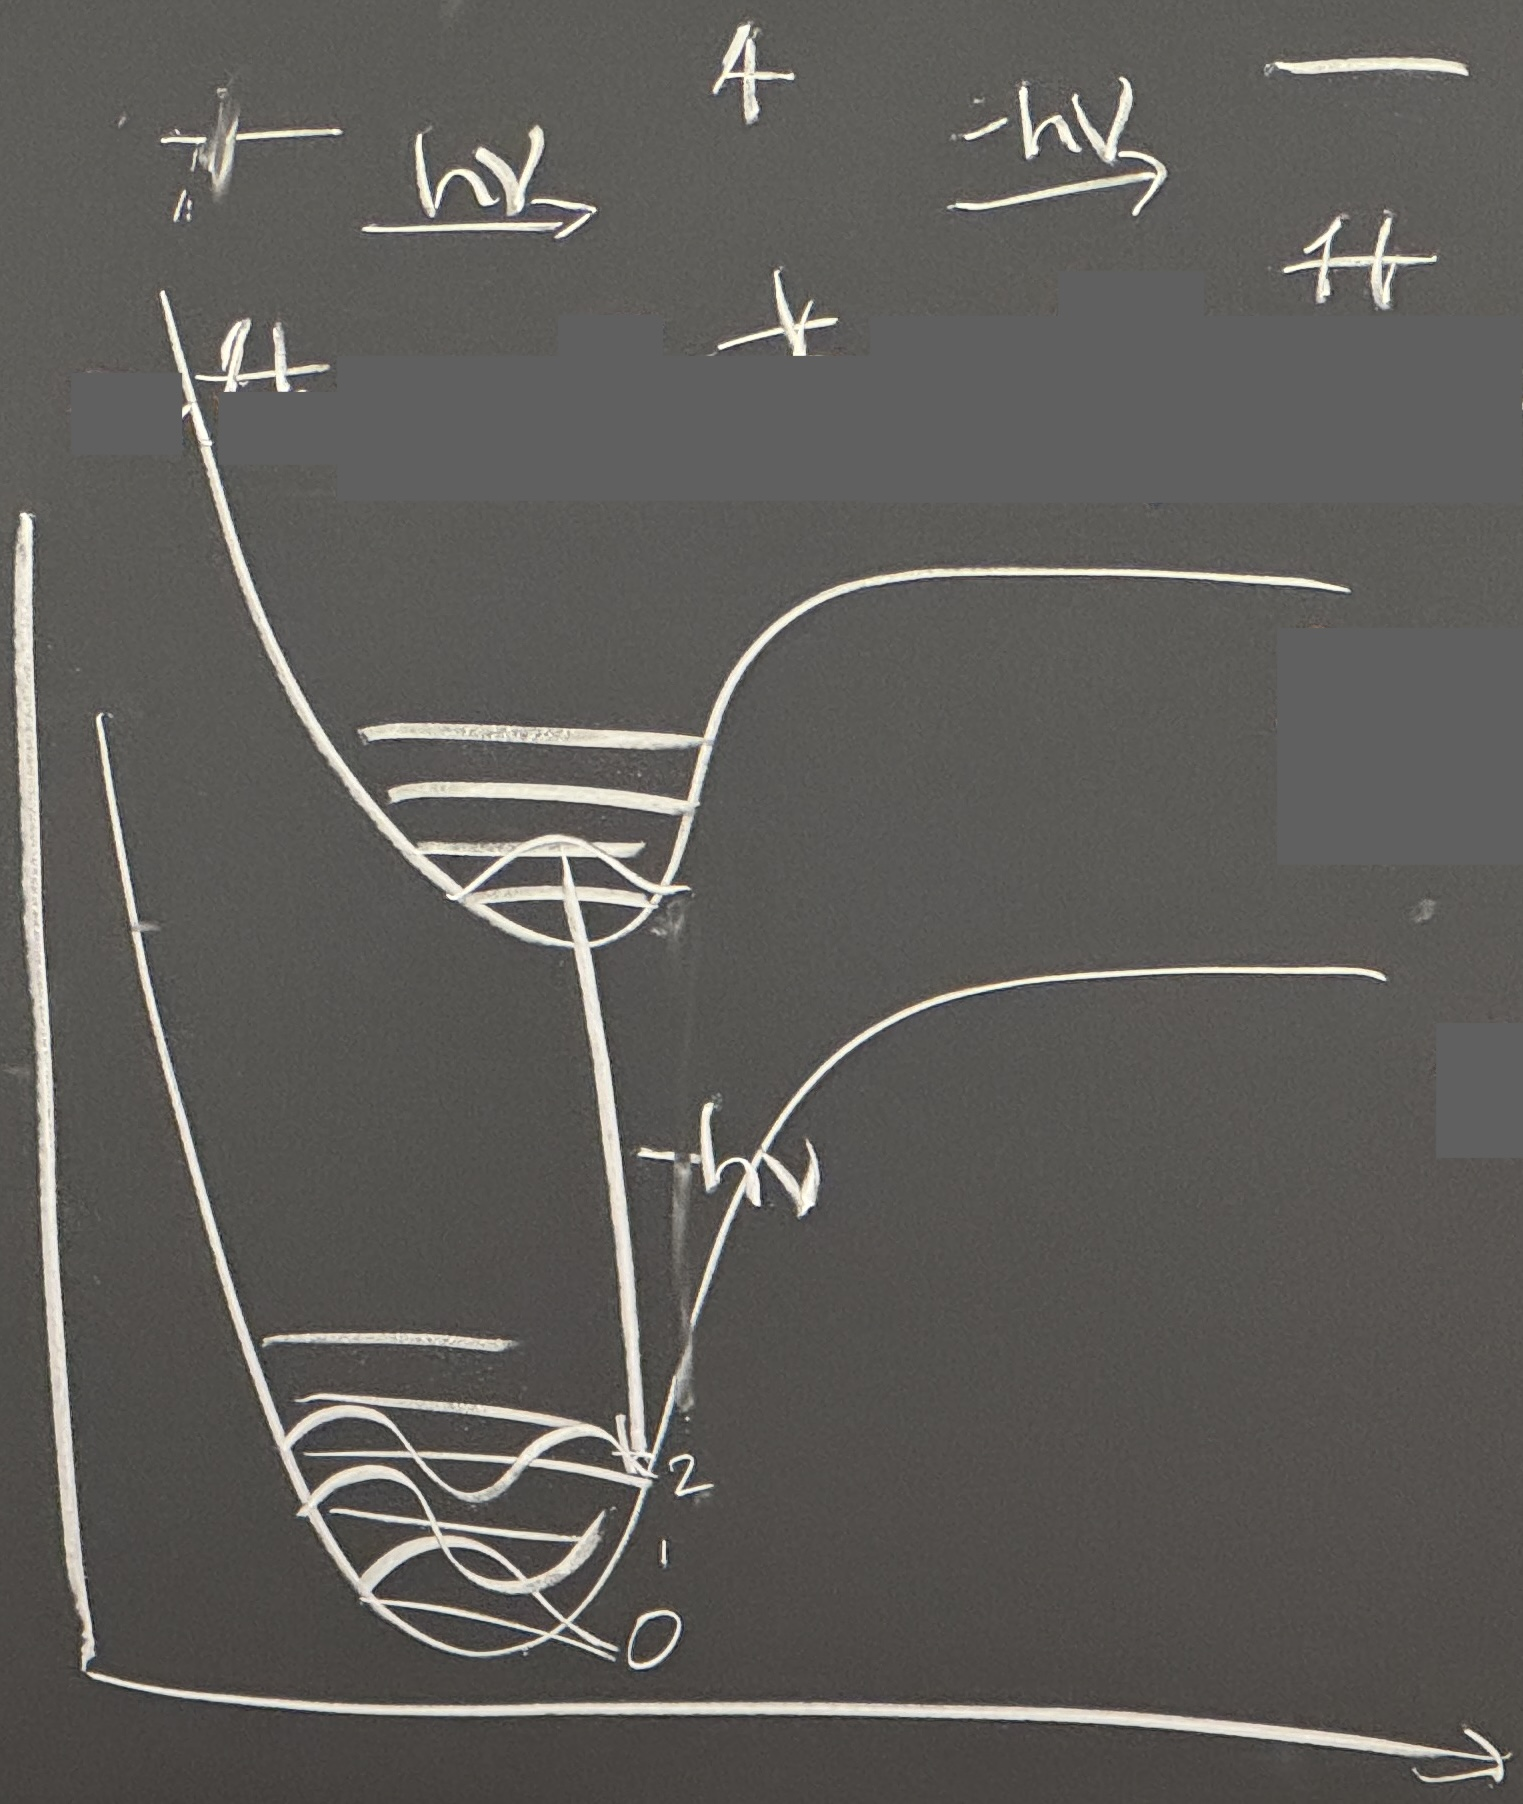
\includegraphics[width=0.85\linewidth]{relaxationMechb.JPG}
            \caption{Fluorescence.}
            \label{fig:relaxationMechb}
        \end{subfigure}
        \begin{subfigure}[b]{0.33\linewidth}
            \centering
            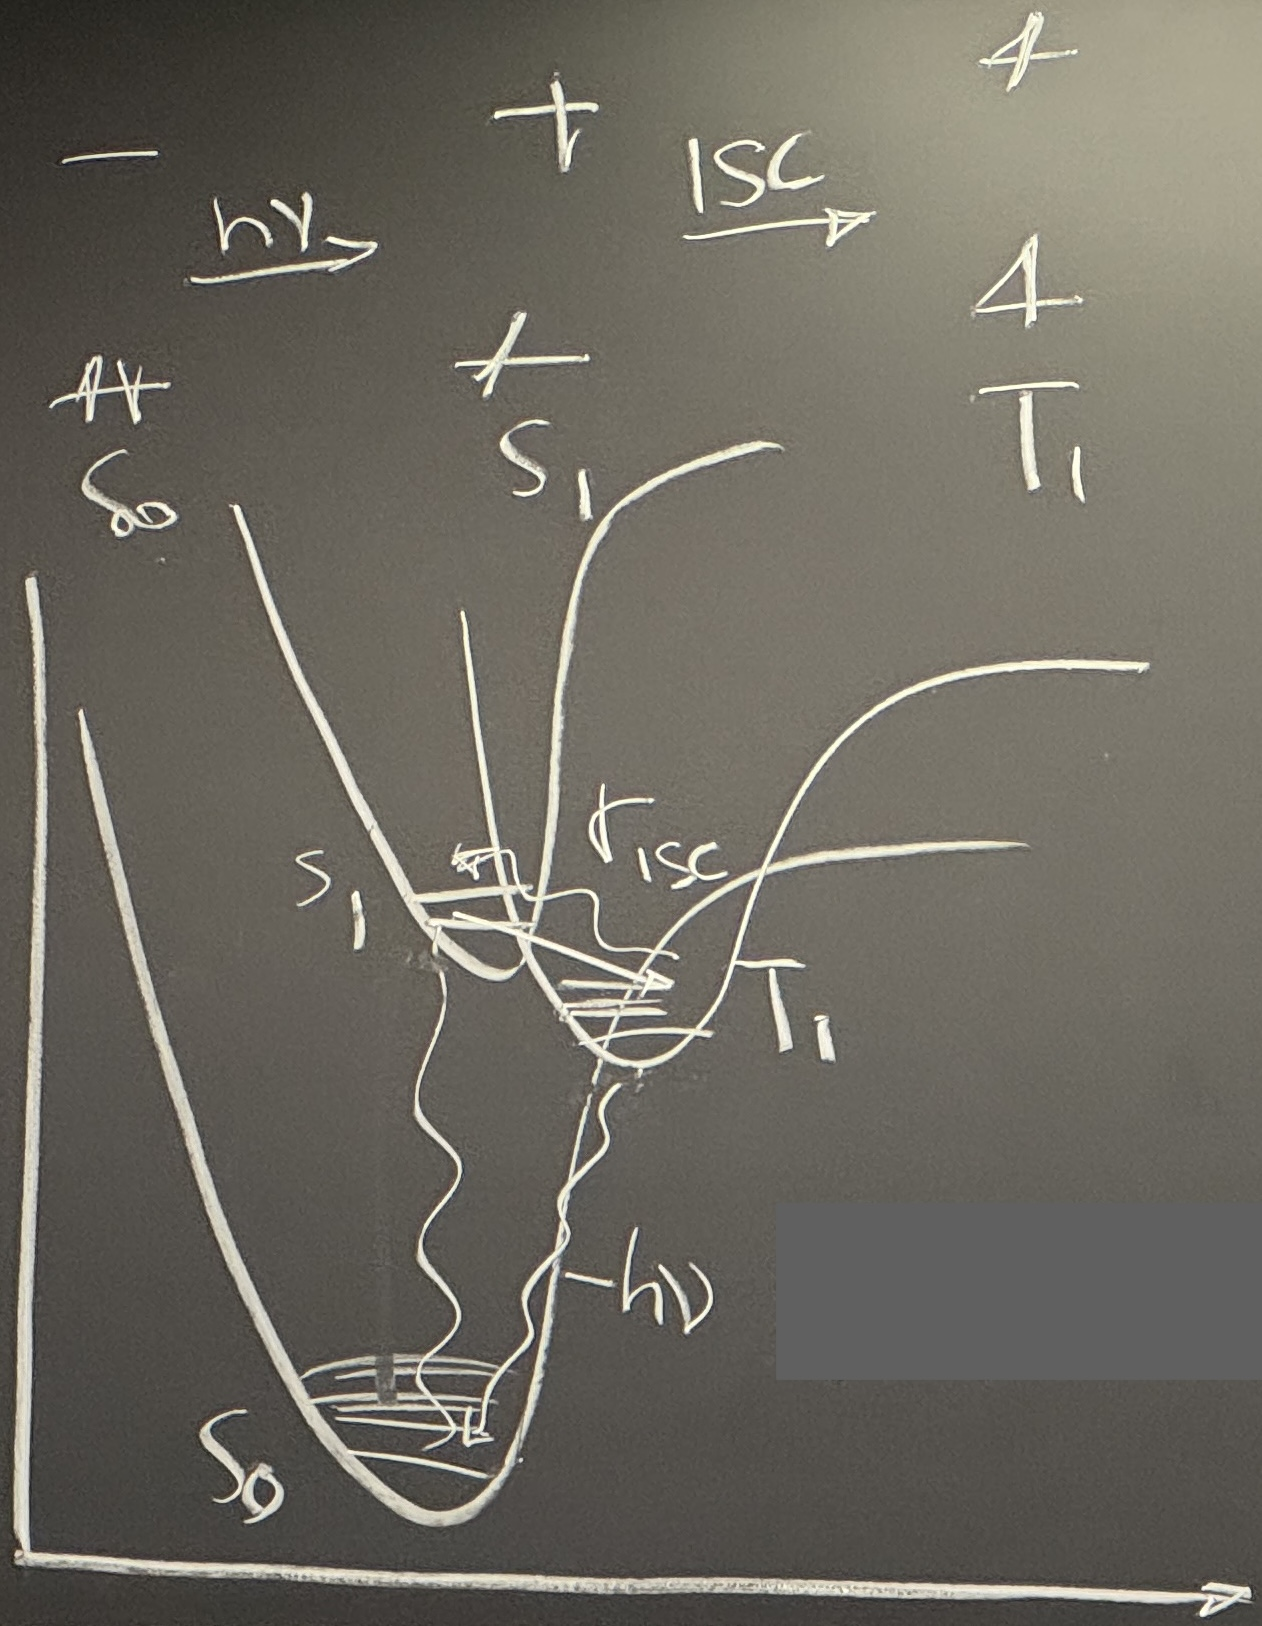
\includegraphics[width=0.85\linewidth]{relaxationMechc.JPG}
            \caption{Phosphorescence.}
            \label{fig:relaxationMechc}
        \end{subfigure}
        \caption{Photochemical relaxation mechanisms.}
        \label{fig:relaxationMech}
    \end{figure}
    \begin{itemize}
        \item Franck-Condon tells us that we can excite into higher vibrational states.
        \begin{itemize}
            \item And we saw previously that we can excite into higher-lying electronic states (e.g., $S_2$).
        \end{itemize}
        \item What happens is answered by \textbf{Kasha's rule}.
        \item Possibility 1: Radiationless decay.
        \begin{itemize}
            \item This is also known as internal conversion.
            \item You can distribute energy to the solvent or else.
            \item This is a mechanism to generate heat from light, and is relatively useless in terms of preparative photochemistry.
            \item So we lose heat to the ground state.
        \end{itemize}
        \item Possibility 2: In the microscopic reverse of absorption, we get Franck-Condon-type emission from the lowest excited vibrational state back down to a higher vibrational ground state.
        \begin{itemize}
            \item This means that we emit a photon of lower energy than we put in!
            \item As drawn, this is $S_1\to S_0$ emission.
            \item Also happens without any change in the angular momentum of the electron.
            \item This is known as fluorescence, and occurs with rate constant $k_f\approx\SIrange{e6}{e9}{\per\second}$.
            \item In the literature, we'll sometimes see a value called the \textbf{fluorescence lifetime}.
            \item So we lose light to the gound state.
        \end{itemize}
        \item Possibility 3: The excited state undergoes intersystem crossing to a triplet excited state ($T_1$).
        \begin{itemize}
            \item Why does this happen?
            \begin{itemize}
                \item Consider the case of benzene.
                \item This does not lead to any bond \emph{cleavage}, but the triplet also has decreased bond order (see Figure \ref{fig:ETDistort}).
                \item By moving electrons out of the same orbital, we remove the Coulombic repulsion. Additionally, since they have the same spin, we benefit from losing the \textbf{Pauli replusion}/gaining the \textbf{exchange energy}. This means that the triplet is slightly lower energy.
            \end{itemize}
            \item But physics hasn't stopped! Where does the momentum go? This has to deal with spin-orbit coupling.
            \begin{itemize}
                \item In much the same way that molecular orbitals of disparate energies don't mix well, the rate of intersystem crossing is also governed by the similarity in energies between $S_1$ and $T_1$; the more similar the energies, the faster ISC happens.
            \end{itemize}
            \item What can the triplet state do?
            \begin{itemize}
                \item It could react right back to the singlet!
                \item This establishes an electronic equilibrium from the singlet and triplet excited states.
                \item The triplet state has a relatively slow rate of electronic emission, but emission from it is called \textbf{phosphorescence}.
                \item Thus, triplet lifetimes are usually many orders of magnitude longer than singlet lifetimes.
                \item Related to TADF organic photoelectronic solar cells.
            \end{itemize}
        \end{itemize}
    \end{itemize}
    \item \textbf{Kasha's rule}: There is a large driving force for relaxation into lower electronic, and vibrational, excited states relative to any other chemistry that may happen.
    \item \textbf{Fluorescence lifetime}: The average time a molecule lives in an excited state before fluorescing. \emph{Denoted by} $\bm{\tau_f}$. \emph{Given by}
    \begin{equation*}
        \tau_f := 1/k_f \approx \frac{10^{-4}}{\epsilon_\text{max}}
    \end{equation*}
    \begin{itemize}
        \item $\epsilon_\text{max}$ is the \textbf{extinction coefficient} from \textbf{Beer's law} ($A=\varepsilon bC$).
        \item This means that in events with strong absorption to the excited state, there's a fast rate at which fluorescence happens.
    \end{itemize}
    \item Example: The photophysics of benzophenone.
    \begin{figure}[H]
        \centering
        \begin{subfigure}[b]{0.38\linewidth}
            \centering
            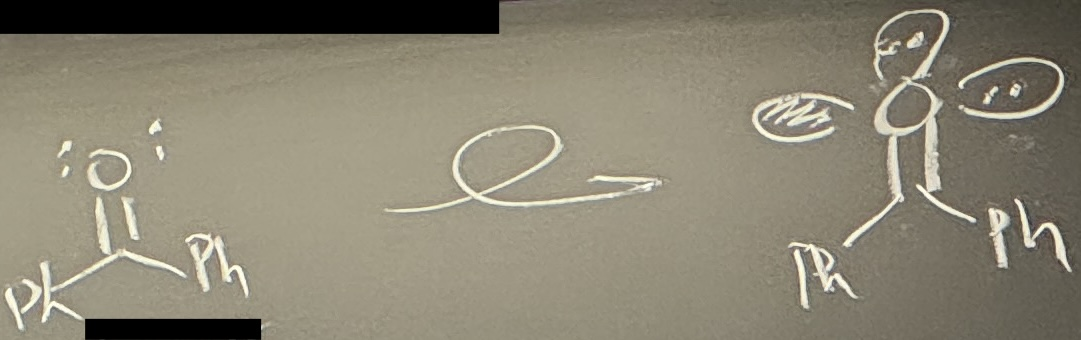
\includegraphics[width=0.75\linewidth]{lightBenzoa.JPG}
            \caption{VSEPR.}
            \label{fig:lightBenzoa}
        \end{subfigure}
        \begin{subfigure}[b]{0.6\linewidth}
            \centering
            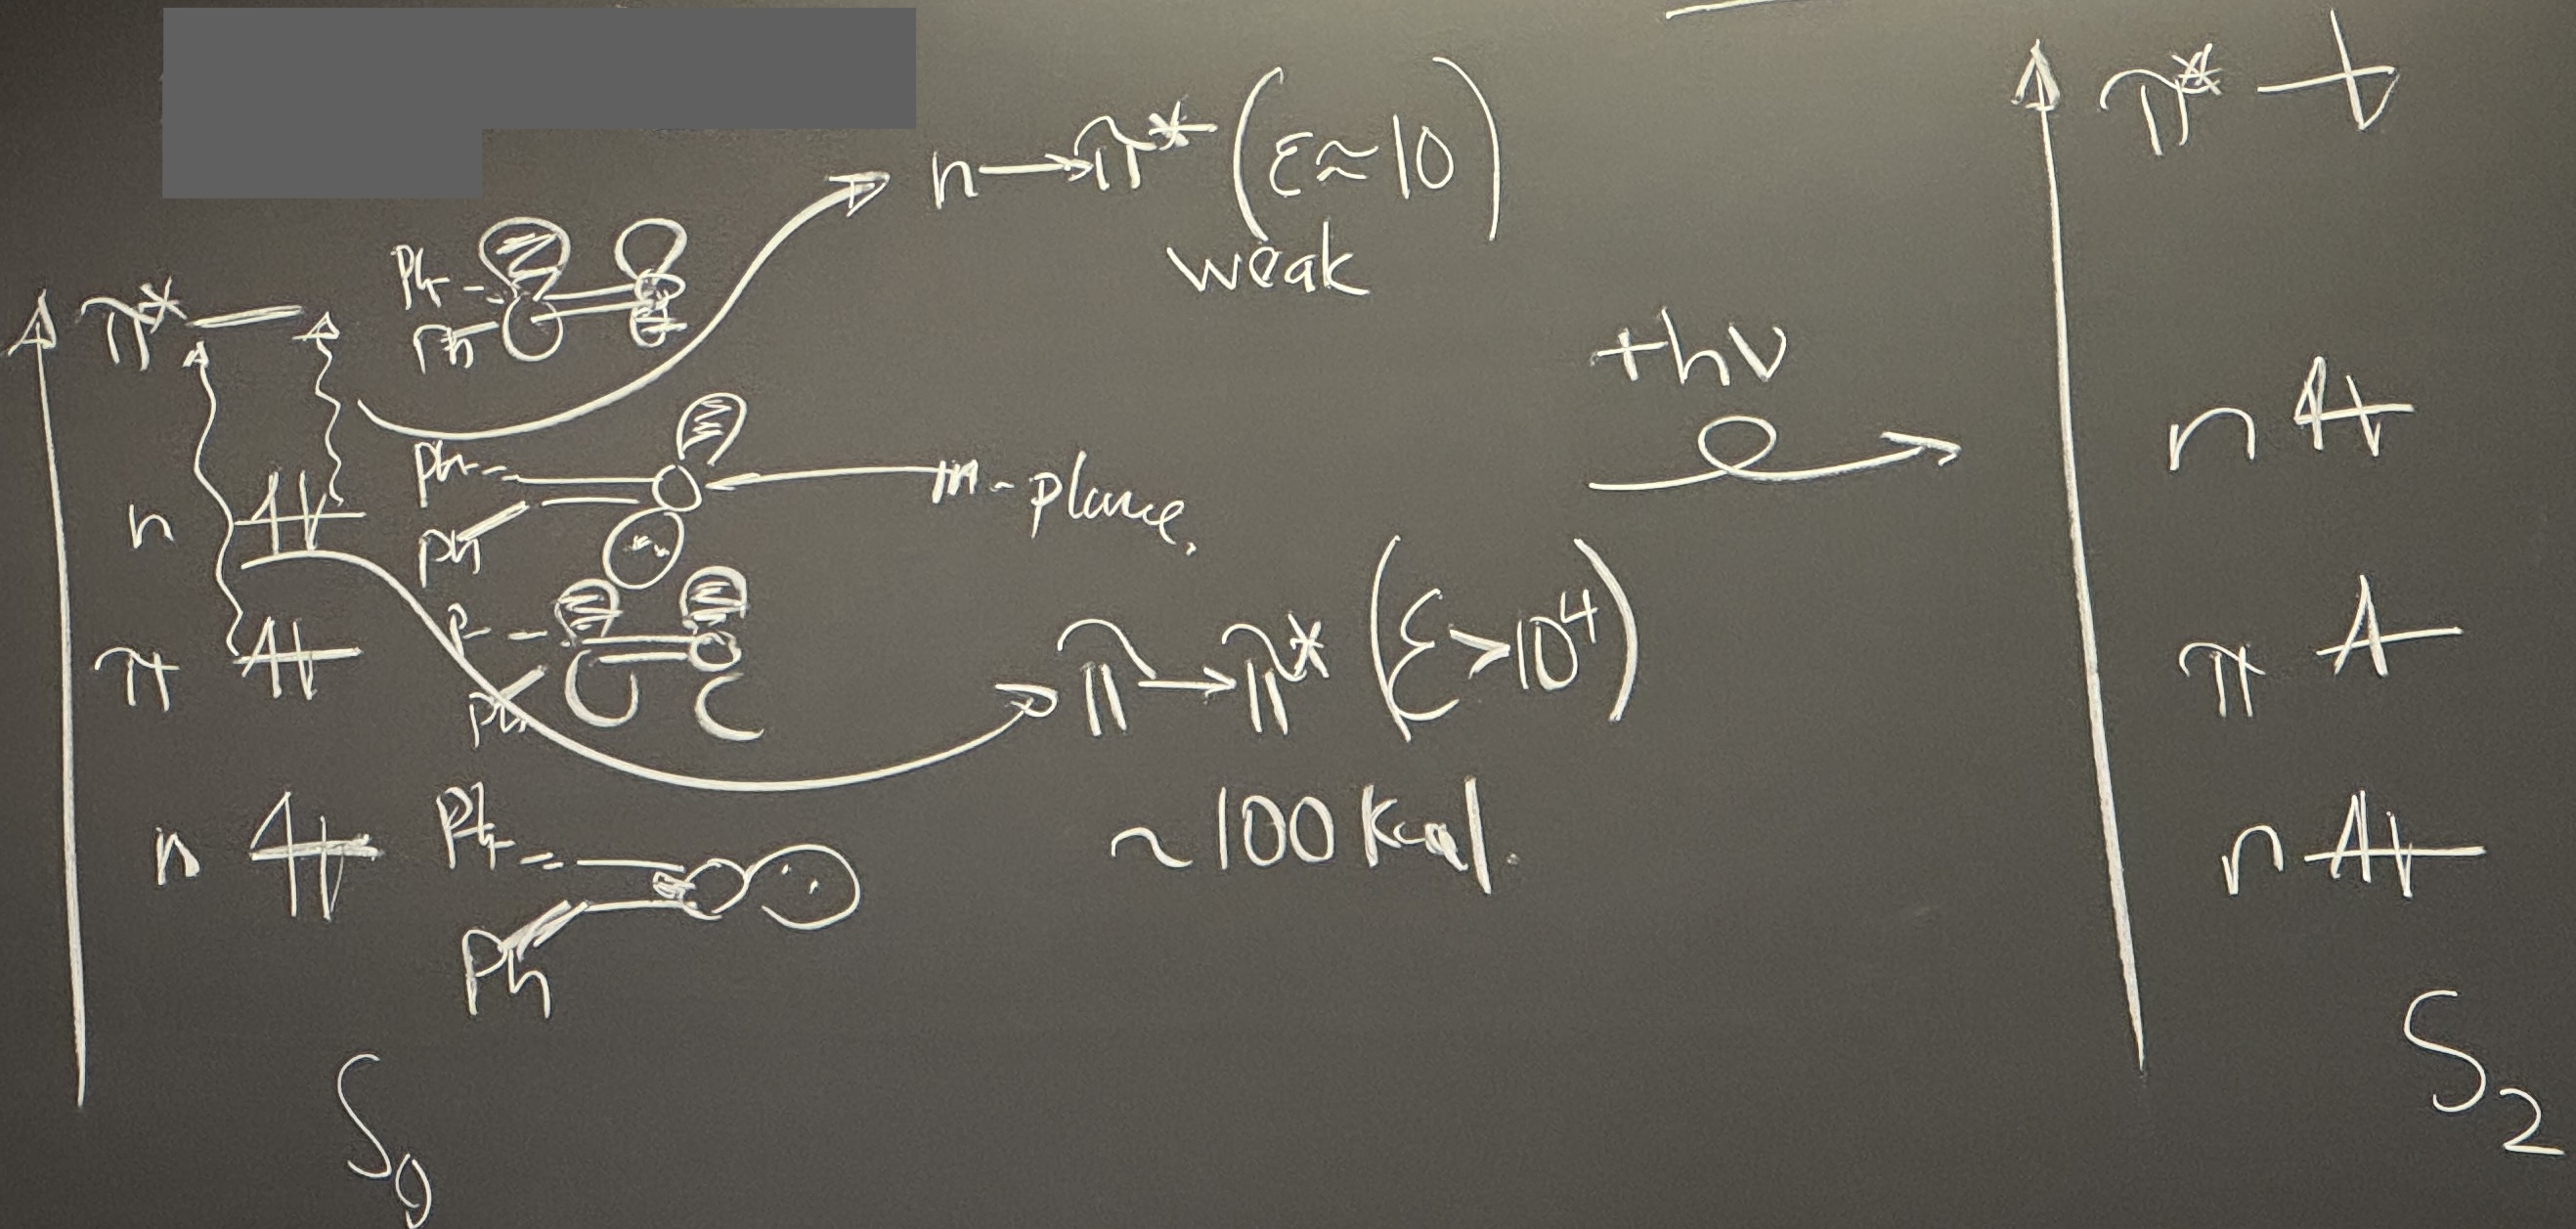
\includegraphics[width=0.95\linewidth]{lightBenzob.JPG}
            \caption{Molecular orbital excitations.}
            \label{fig:lightBenzob}
        \end{subfigure}
        \caption{Electronic structure of benzophenone.}
        \label{fig:lightBenzo}
    \end{figure}
    \begin{itemize}
        \item The frontier MOs are the carbonyl $\pi$ and $\pi^*$ orbitals.
        \item It's also got nonbonding lone pairs on the oxygen.
        \begin{itemize}
            \item An $sp$-hybridized oxygen is more likely than an $sp^2$-hybridize one: One lone pair in $sp$ and one in an orthogonal $p$-orbital.
            \item These two nonbonding pairs are nondegenerate: This is molecular orbital theory, as in the nonequivalent electron pairs of \ce{H2O} (see Figure III.12 from \textcite{bib:CHEM20100Notes}).
            \item Technically, this is an excuse by VSEPR purists!
        \end{itemize}
        \item Consider an $n\to\pi^*$ transition.
        \begin{itemize}
            \item Because there is very little orbital overlap, we have an extinction coefficient of $\varepsilon\approx 10$. Thus, this is a weak transition with little absorption, so it tends not to be important and the context of benzophenone.
        \end{itemize}
        \item Consider the $\pi\to\pi^*$ transition.
        \begin{itemize}
            \item Here, $\varepsilon>10^4$.
            \item Thus, we'll preferentially excite this transition.
            \item The $\lambda_\text{max}$ for this transition is known; we can look up the exact value, but it's about \SI{315}{\nano\meter}.
            \item In effect, the result is an $S_2$ state because we've excited up two energy levels.
        \end{itemize}
    \end{itemize}
    \item Let's now look at a diagram that is rigorous energetically but dispenses with the internuclear coordinate. This is a \textbf{Jablonski diagram}.
    \begin{figure}[H]
        \centering
        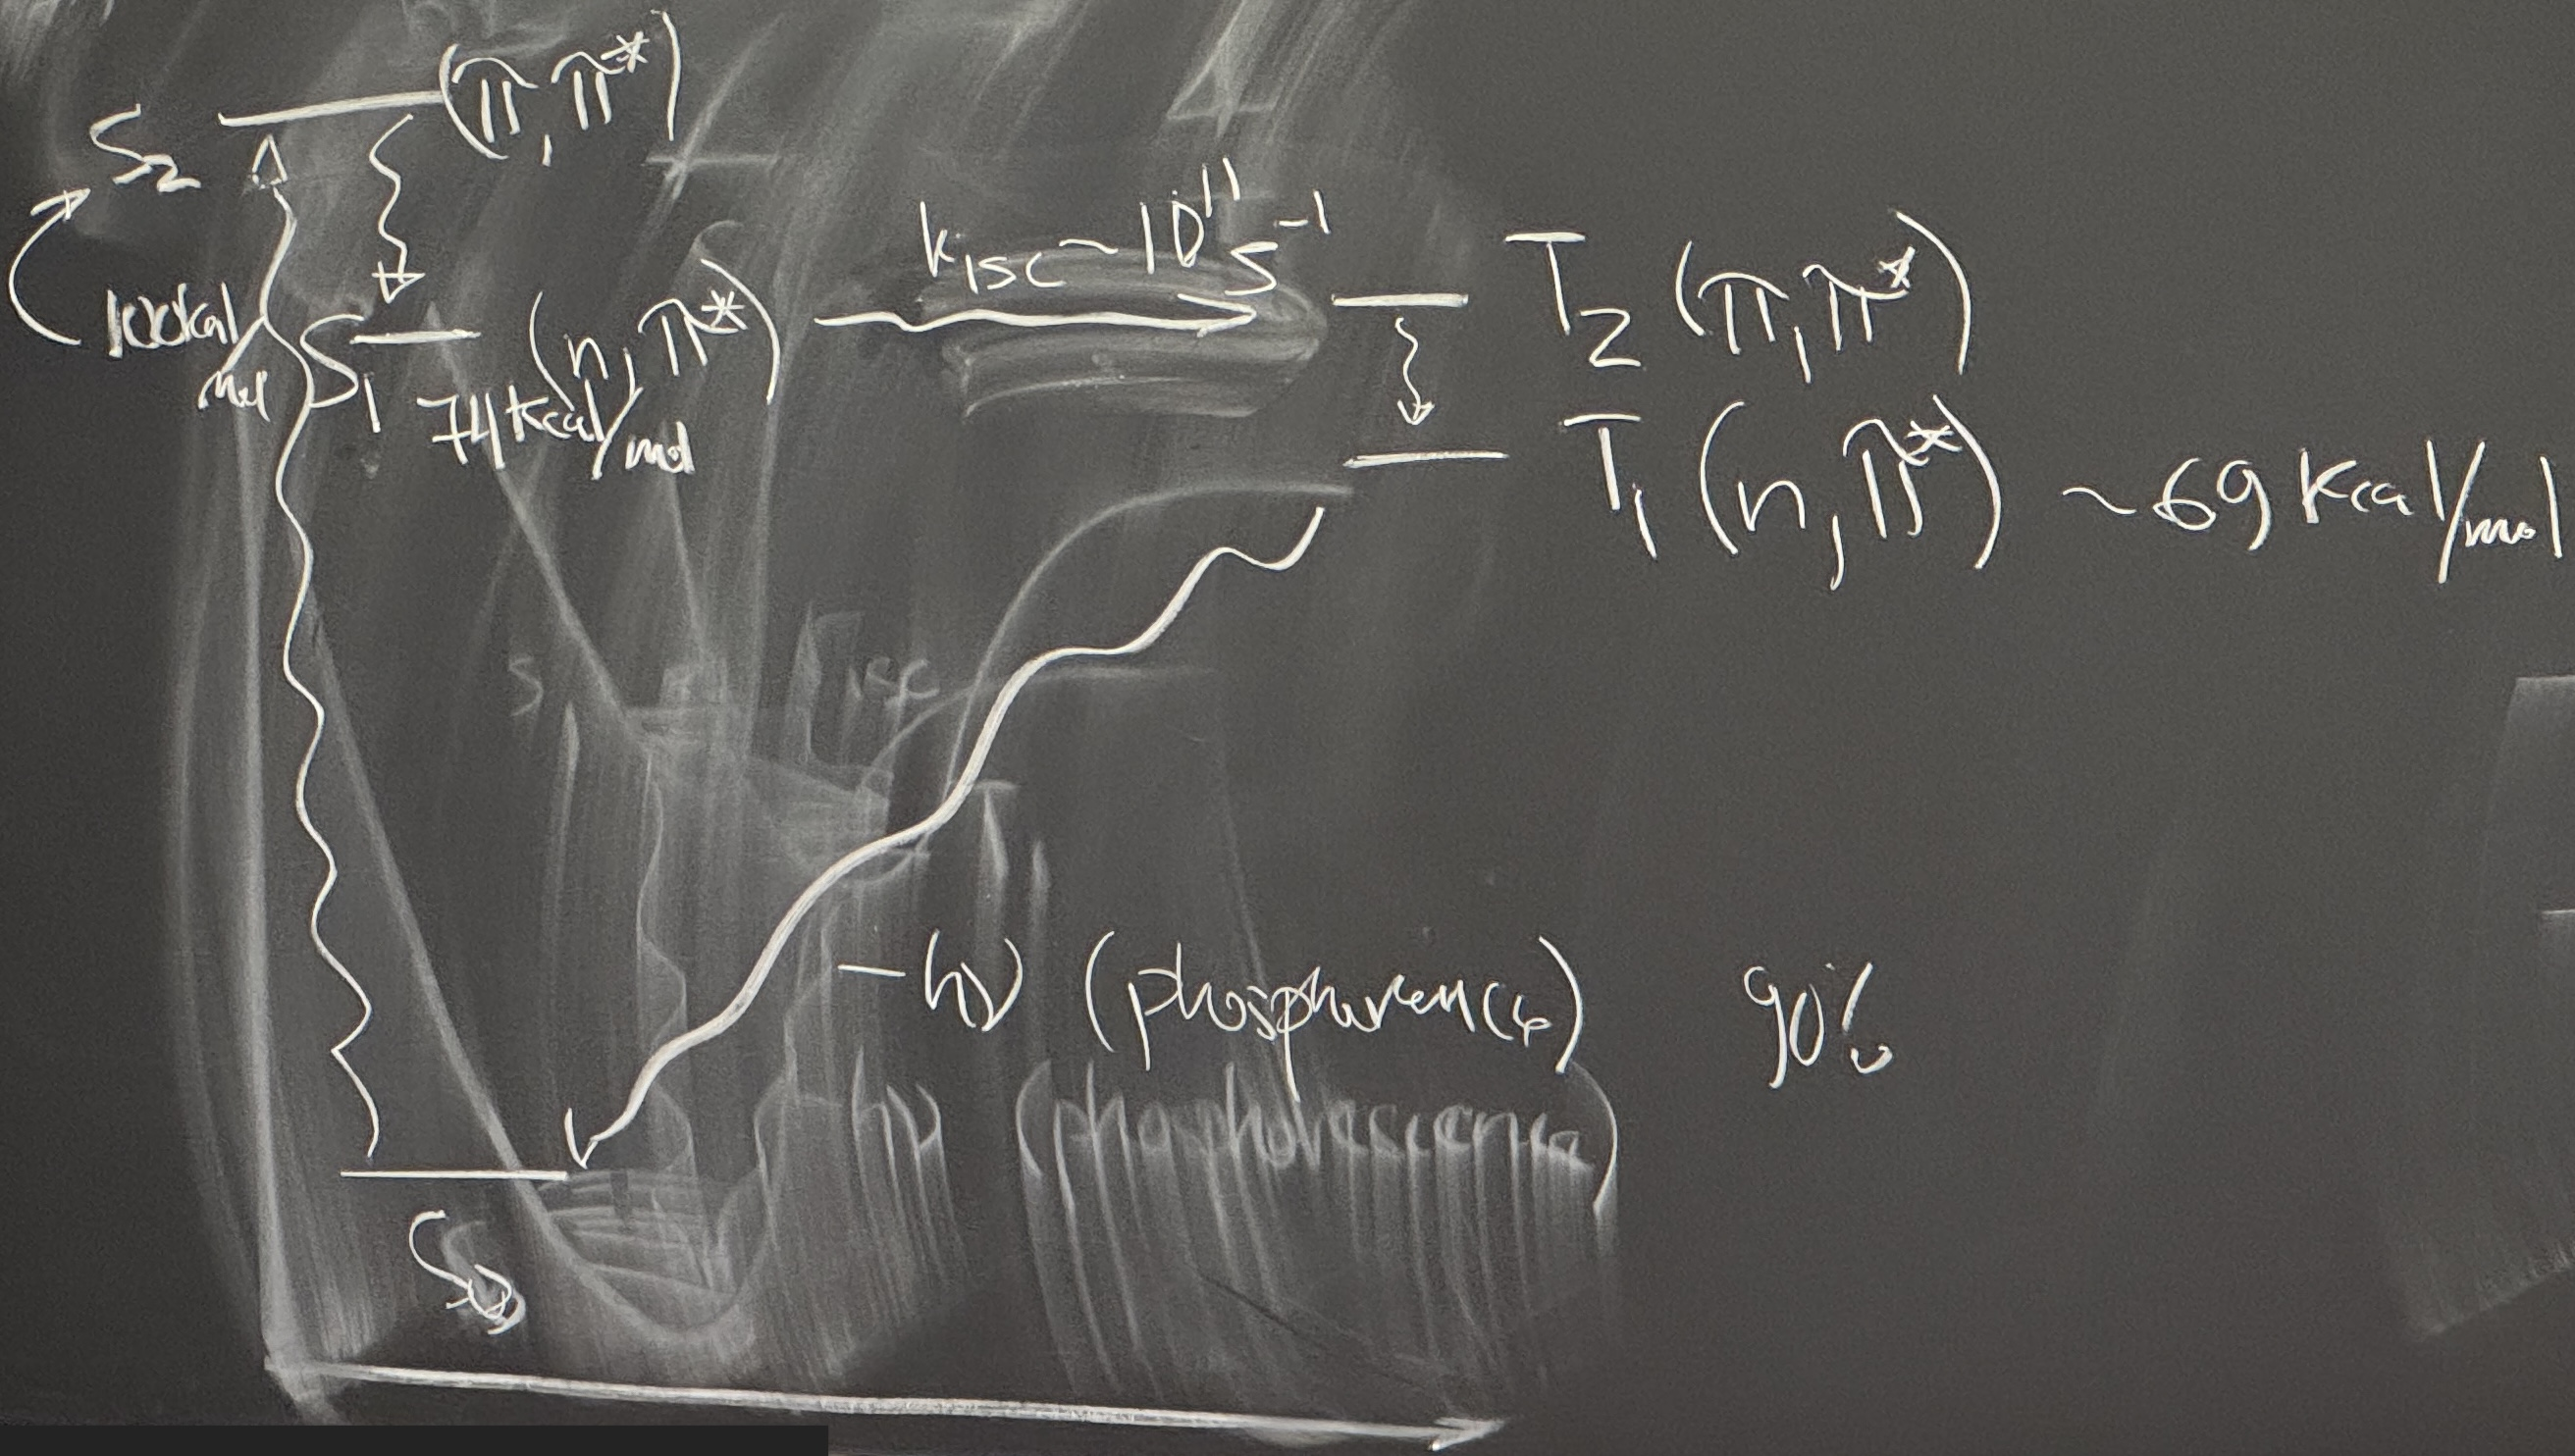
\includegraphics[width=0.6\linewidth]{JabBenzo.JPG}
        \caption{Jablonski diagram for exciting benzophenone.}
        \label{fig:JabBenzo}
    \end{figure}
    \begin{itemize}
        \item Excitation to $S_2$ happens with an energy of about \kcal{100}. Occurs with a $(\pi,\pi^*)$ transition.
        \item This then follows with rapid relaxation to the $S_1$ singlet.
        \begin{itemize}
            \item This new $S_1$ state is lower in energy, electronically.
            \item We can also show this on our Jablonski diagram!
            \item $S_1$ is at \kcal{74}, experimentally.
            \item Fluorescence from $S_1$ (in a right angle array; spectrofluorophotometry!) experimentally gives you the energy of this state.
        \end{itemize}
        \item Very fast intersystem crossing ($k_\text{ISC}\approx\SI{e11}{\per\second}$) from $S_1\to T_2$ can then occur.
        \begin{itemize}
            \item This is because the $T_2$ state happens to be very similar in energy to $S_1$.
        \end{itemize}
        \item Then we quickly drop to $T_1$.
        \begin{itemize}
            \item We can hang here for a while; long lifetime.
            \item Triplets are spin-forbidden to go down to the ground state, with lifetimes on milliseconds to even seconds.
            \item This lifetime is comparable to diffusion, so we can do chemistry now!
        \end{itemize}
        \item Alternatively, phosphorescence back to the ground state.
        \begin{itemize}
            \item 90\% of the energy goes here.
        \end{itemize}
    \end{itemize}
    \item We care about benzophenone because it's oft-used in preparative photochemistry as a triplet sensitizer.
    \item Photochemistry.
    \item Intermolecular energy transfer can occur.
    \begin{figure}[h!]
        \centering
        \begin{subfigure}[b]{0.35\linewidth}
            \centering
            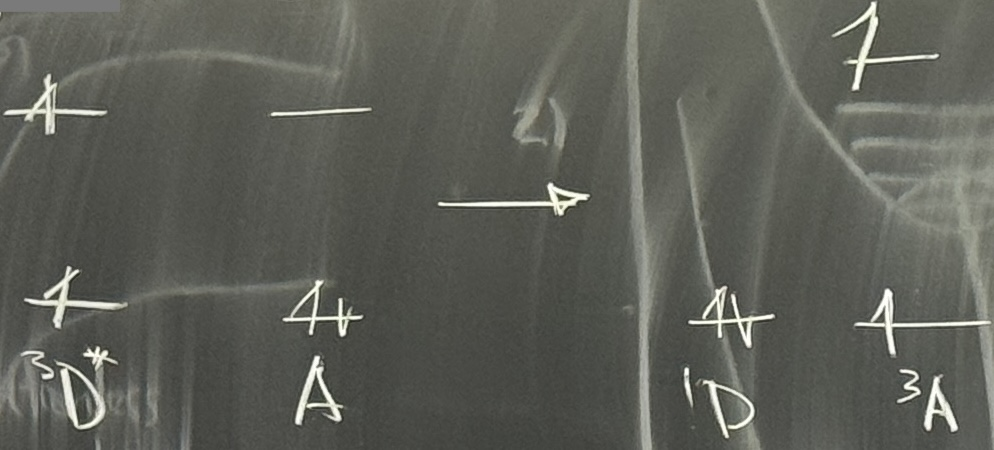
\includegraphics[width=0.8\linewidth]{photochema.JPG}
            \caption{Dexter energy transfer.}
            \label{fig:photochema}
        \end{subfigure}
        \begin{subfigure}[b]{0.35\linewidth}
            \centering
            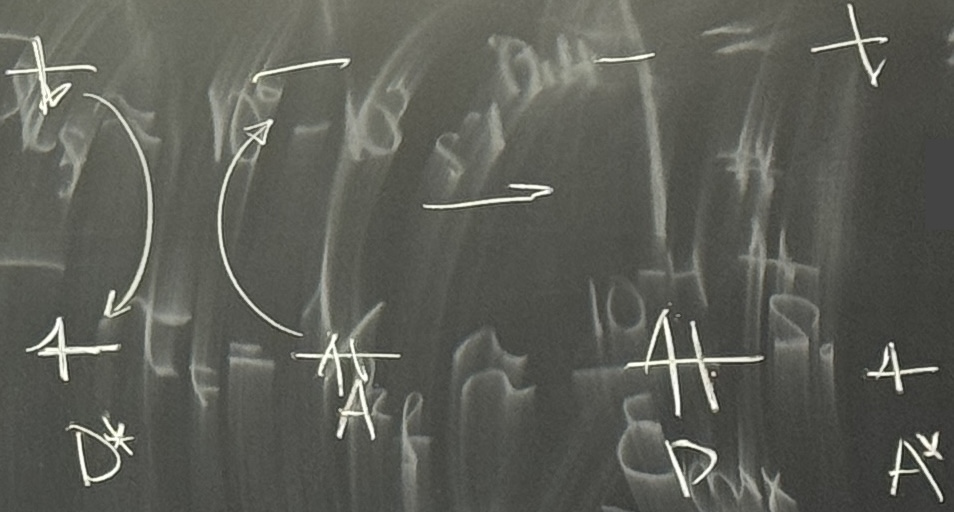
\includegraphics[width=0.8\linewidth]{photochemb.JPG}
            \caption{Forster energy transfer.}
            \label{fig:photochemb}
        \end{subfigure}\\[2em]
        \begin{subfigure}[b]{\linewidth}
            \centering
            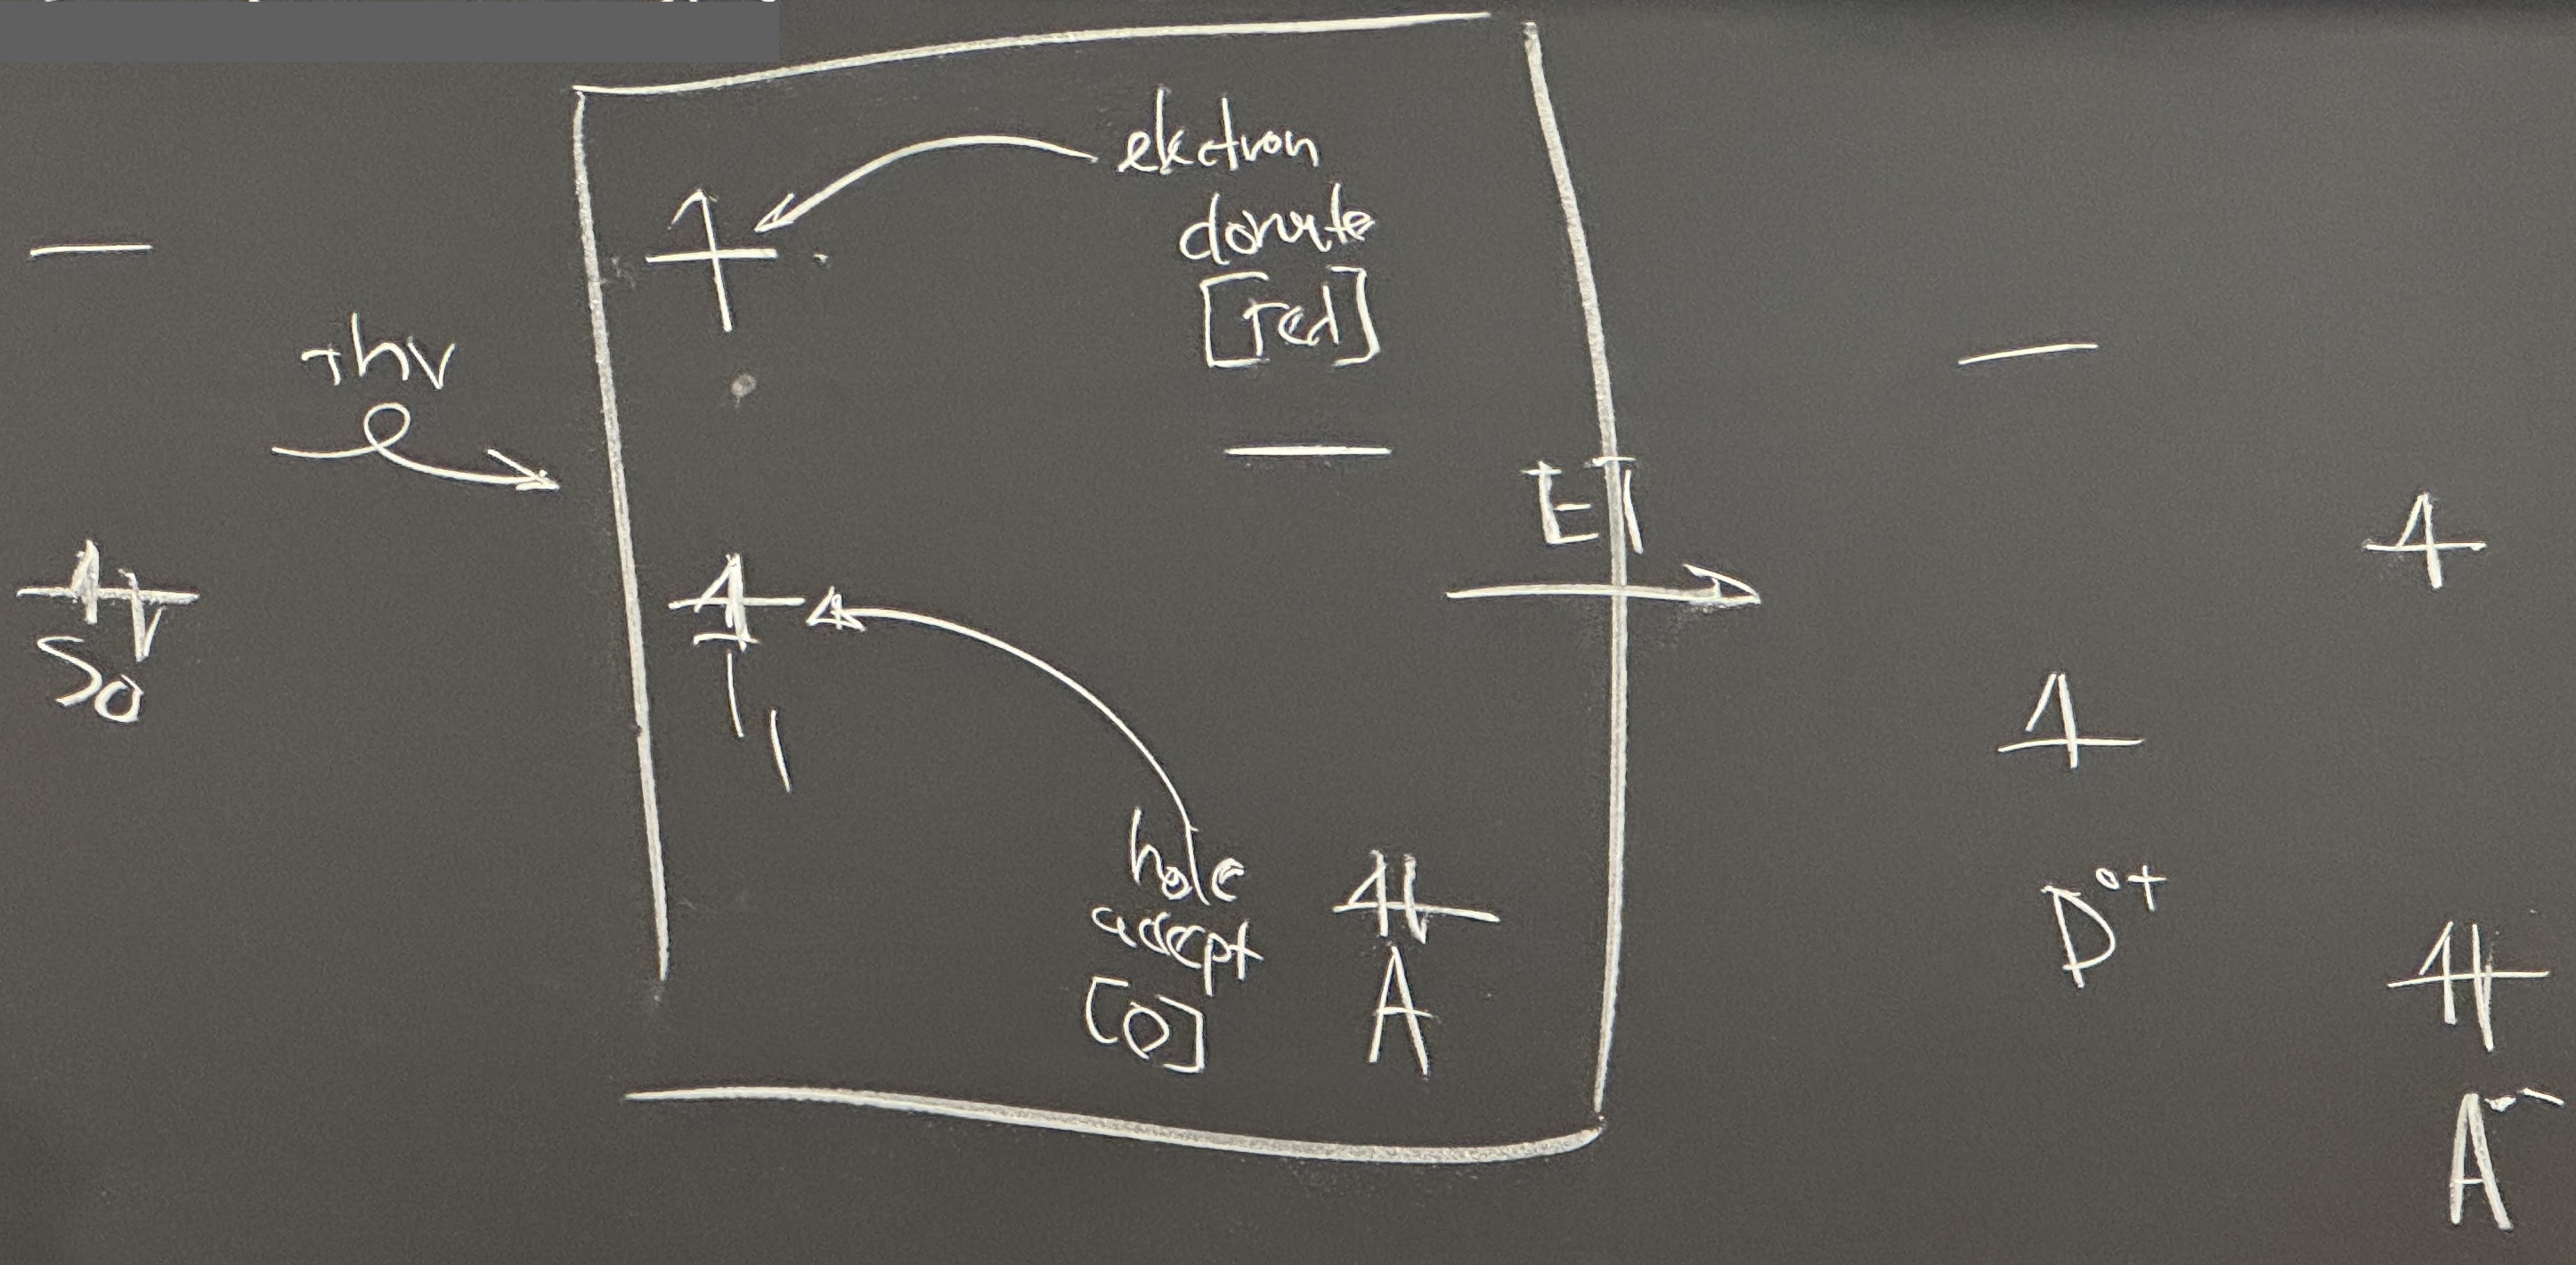
\includegraphics[width=0.5\linewidth]{photochemc.JPG}
            \caption{Electron transfer.}
            \label{fig:photochemc}
        \end{subfigure}
        \caption{Intermolecular photochemistry.}
        \label{fig:photochem}
    \end{figure}
    \begin{enumerate}
        \item Donor to acceptor (\ce{D^* + A -> D + A^*}).
        \begin{enumerate}
            \item Dexter energy transfer.
            \begin{itemize}
                \item The triplet excited state relaxes to its singlet and excites the acceptor to its triplet.
                \item Example: Triplet benzophenone and singlet naphthalene transfers to singlet benzophenone and triplet naphthalene.
            \end{itemize}
            \item Forster energy transfer.
            \begin{itemize}
                \item Energy falling down causes energy up in the acceptor.
                \item The rate here is exquisitely dependent on distance ($k_\text{For}\propto1/r^6$).
                \item This type of transfer relies on good orbital overlap between the donor and acceptor.
            \end{itemize}
        \end{enumerate}
        \item Electron transfer.
        \begin{itemize}
            \item A hole can accept electrons from another molecule (oxidation), and the excited electron can donate (reduction).
            \begin{itemize}
                \item Takeaway: Photoexcited species are better both donors and acceptors.
            \end{itemize}
            \item Hole transfer creates a radical cation and radical anion.
        \end{itemize}
    \end{enumerate}
    \item Stuff Alex didn't get to: Stern-Volmer quenching, excited state electron transfer, mechanisms of photoisomerization, and photoluminescence.
    \item Closing thoughts.
    \begin{itemize}
        \item Graduate education is a fraught transitional process from learning other people's knowledge to generating your own knowledge.
        \item Alex is eager to be a resource to us in future years; door is open.
        \item He also hopes to learn from us, because we know some things better than he ever will.
    \end{itemize}
\end{itemize}




\end{document}